% Fig. 1 teaser, UGG-idea variant, WIDE layout (2026-11-13; user: "try to make it wider so that it will take less
% space"). One row instead of two: the two row photographs (sorghum, maize) -> the model -> the two centre plants'
% procedural parameters. At \textwidth it is ~40 % of the two-row version's height; type sizes raised so the printed
% sizes match the two-row version. Not used by main.tex (which inputs Figures/fig_teaser_tikz).
% Conventions from the UGG paper (Unified Generative Geometry Model): one pastel colour per stream (image blue,
% parameters purple), inputs in dashed rounded boxes, outputs solid, a model block with a soft gradient through the
% stream colours and a dashed rule, one grey frame around what the model writes, grey block arrows. Font: \sffamily
% (Helvetica under the cvpr/times package), as the paper's teaser.
% Content (user, 2026-11-13): header "Model"; the output is the procedural parameters only, drawn as in the
% any-to-all figure (figures/make_teaser_recipe_tiles.py: the written recipe in purple over the true one in grey),
% no value text. Plants: the held-out test rows of figures/make_teaser_v2.py --mode row (Sorghum_10113, plant_0106).
% Include with \resizebox{\textwidth}{!}{% Fig. 1 teaser, UGG-idea variant, WIDE layout (2026-11-13; user: "try to make it wider so that it will take less
% space"). One row instead of two: the two row photographs (sorghum, maize) -> the model -> the two centre plants'
% procedural parameters. At \textwidth it is ~40 % of the two-row version's height; type sizes raised so the printed
% sizes match the two-row version. Not used by main.tex (which inputs Figures/fig_teaser_tikz).
% Conventions from the UGG paper (Unified Generative Geometry Model): one pastel colour per stream (image blue,
% parameters purple), inputs in dashed rounded boxes, outputs solid, a model block with a soft gradient through the
% stream colours and a dashed rule, one grey frame around what the model writes, grey block arrows. Font: \sffamily
% (Helvetica under the cvpr/times package), as the paper's teaser.
% Content (user, 2026-11-13): header "Model"; the output is the procedural parameters only, drawn as in the
% any-to-all figure (figures/make_teaser_recipe_tiles.py: the written recipe in purple over the true one in grey),
% no value text. Plants: the held-out test rows of figures/make_teaser_v2.py --mode row (Sorghum_10113, plant_0106).
% Include with \resizebox{\textwidth}{!}{% Fig. 1 teaser, UGG-idea variant, WIDE layout (2026-11-13; user: "try to make it wider so that it will take less
% space"). One row instead of two: the two row photographs (sorghum, maize) -> the model -> the two centre plants'
% procedural parameters. At \textwidth it is ~40 % of the two-row version's height; type sizes raised so the printed
% sizes match the two-row version. Not used by main.tex (which inputs Figures/fig_teaser_tikz).
% Conventions from the UGG paper (Unified Generative Geometry Model): one pastel colour per stream (image blue,
% parameters purple), inputs in dashed rounded boxes, outputs solid, a model block with a soft gradient through the
% stream colours and a dashed rule, one grey frame around what the model writes, grey block arrows. Font: \sffamily
% (Helvetica under the cvpr/times package), as the paper's teaser.
% Content (user, 2026-11-13): header "Model"; the output is the procedural parameters only, drawn as in the
% any-to-all figure (figures/make_teaser_recipe_tiles.py: the written recipe in purple over the true one in grey),
% no value text. Plants: the held-out test rows of figures/make_teaser_v2.py --mode row (Sorghum_10113, plant_0106).
% Include with \resizebox{\textwidth}{!}{% Fig. 1 teaser, UGG-idea variant, WIDE layout (2026-11-13; user: "try to make it wider so that it will take less
% space"). One row instead of two: the two row photographs (sorghum, maize) -> the model -> the two centre plants'
% procedural parameters. At \textwidth it is ~40 % of the two-row version's height; type sizes raised so the printed
% sizes match the two-row version. Not used by main.tex (which inputs Figures/fig_teaser_tikz).
% Conventions from the UGG paper (Unified Generative Geometry Model): one pastel colour per stream (image blue,
% parameters purple), inputs in dashed rounded boxes, outputs solid, a model block with a soft gradient through the
% stream colours and a dashed rule, one grey frame around what the model writes, grey block arrows. Font: \sffamily
% (Helvetica under the cvpr/times package), as the paper's teaser.
% Content (user, 2026-11-13): header "Model"; the output is the procedural parameters only, drawn as in the
% any-to-all figure (figures/make_teaser_recipe_tiles.py: the written recipe in purple over the true one in grey),
% no value text. Plants: the held-out test rows of figures/make_teaser_v2.py --mode row (Sorghum_10113, plant_0106).
% Include with \resizebox{\textwidth}{!}{\input{Figures/fig_teaser_tikz_ugg}} (needs \usetikzlibrary{arrows.meta}).
\definecolor{tInk}{HTML}{1D221C}\definecolor{tMuted}{HTML}{5F685C}%
\definecolor{uRgbE}{HTML}{809EC2}\definecolor{uRgbF}{HTML}{E6ECF3}\definecolor{uRgbI}{HTML}{3F5F8F}%
\definecolor{uPcF}{HTML}{F6E9ED}\definecolor{uDepF}{HTML}{FAF2D4}%
\definecolor{uTxE}{HTML}{9D8CC4}\definecolor{uTxF}{HTML}{EAE7F2}\definecolor{uTxI}{HTML}{5E4A96}%
\definecolor{uOutE}{HTML}{B4B4B8}\definecolor{uArrow}{HTML}{8C8C8C}\definecolor{uModE}{HTML}{9A9A9A}%
\pgfdeclarehorizontalshading{uggband}{100bp}{color(0bp)=(uRgbF); color(30bp)=(uRgbF); color(45bp)=(uDepF); color(60bp)=(uPcF); color(75bp)=(uTxF); color(100bp)=(uTxF)}%
\begin{tikzpicture}[x=0.005in, y=-0.005in]
\useasboundingbox (0,0) rectangle (1320,340);
\tikzset{hdr/.style={anchor=center, inner sep=0, align=center, font={\fontsize{8.5}{10.2}\selectfont\sffamily\bfseries}},
         sp/.style={anchor=base, inner sep=0, align=center, text=tInk, font={\fontsize{7.2}{8.6}\selectfont\sffamily\bfseries}},
         tcap/.style={anchor=north, inner sep=0, align=center, text=tMuted, font={\fontsize{5.6}{6.8}\selectfont\sffamily}},
         blk/.style={color=uArrow, line width=3.0pt, -{Triangle[length=5.5pt,width=8.5pt]}}}
% ---- headers ----
\node[hdr, text=uRgbI] at (260.0,18.0) {Image of an occluded crop row (input)};
\node[hdr, text=tInk] at (662.0,18.0) {Model};
\node[hdr, text=uTxI] at (1055.0,18.0) {Procedural parameters of the center plant};
% ---- inputs: the row photographs ----
\node[sp] at (136.0,56.0) {sorghum};
\node[sp] at (384.0,56.0) {maize};
\draw[draw=uRgbE, line width=1.0pt, rounded corners=6.5pt, fill=uRgbF, dash pattern=on 3pt off 2pt] (20.0,68.0) rectangle (252.0,300.0);
\node[anchor=north west, inner sep=0] at (26.0,74.0) {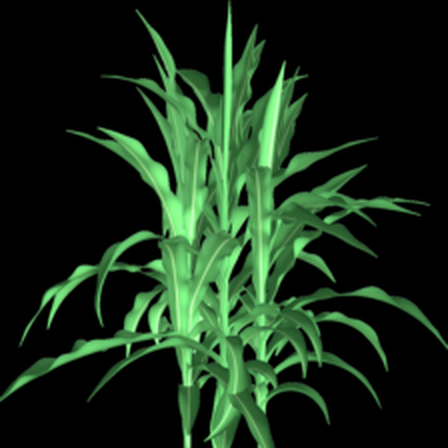
\includegraphics[width=1.1000in, height=1.1000in]{Figures/teaser/s_rgb.png}};
\draw[draw=white, densely dashed, line width=0.80pt] (104.0,88.0) rectangle (168.0,284.0);
\node[anchor=north west, inner sep=1.5pt, text=white, font={\fontsize{5.0}{6.0}\selectfont\sffamily\bfseries}] at (104.0,88.0) {target plant};
\node[tcap] at (136.0,308.0) {25\,\% hidden by neighbours};
\draw[draw=uRgbE, line width=1.0pt, rounded corners=6.5pt, fill=uRgbF, dash pattern=on 3pt off 2pt] (268.0,68.0) rectangle (500.0,300.0);
\node[anchor=north west, inner sep=0] at (274.0,74.0) {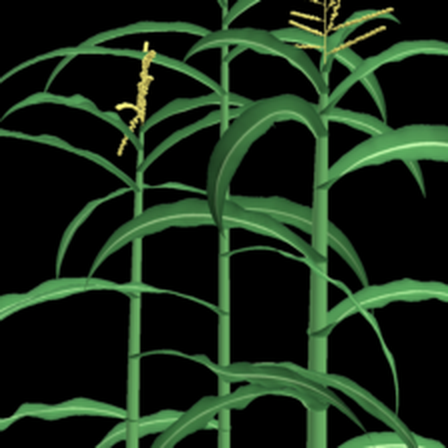
\includegraphics[width=1.1000in, height=1.1000in]{Figures/teaser/m_rgb.png}};
\draw[draw=white, densely dashed, line width=0.80pt] (354.0,84.0) rectangle (430.0,290.0);
\node[anchor=north west, inner sep=1.5pt, text=white, font={\fontsize{4.6}{5.6}\selectfont\sffamily\bfseries}] at (354.0,84.0) {target plant};
\node[tcap] at (384.0,308.0) {22\,\% hidden by neighbours};
\draw[blk] (510.0,184.0) -- (566.0,184.0);
% ---- the model ----
\draw[draw=uModE, line width=1.0pt, rounded corners=8.6pt, shading=uggband, shading angle=0] (574.0,68.0) rectangle (750.0,300.0);
\node[anchor=center, inner sep=0, text=tInk, font={\fontsize{9.0}{10.8}\selectfont\sffamily\bfseries}] at (662.0,120.0) {CropCode};
\draw[draw=uModE, line width=0.6pt, dash pattern=on 2.2pt off 1.6pt] (600.0,146.0) -- (724.0,146.0);
\node[anchor=north, inner sep=0, align=center, text=tInk, font={\fontsize{5.3}{6.6}\selectfont\sffamily}] at (662.0,166.0) {any-to-any\\autoencoder over\\photographs, depth,\\clouds and recipes;\\pretrained on single\\plants, fine-tuned\\on crop rows};
\draw[blk] (758.0,184.0) -- (806.0,184.0);
% ---- outputs: the procedural parameters ----
\draw[draw=uOutE, line width=0.9pt, rounded corners=8.6pt] (814.0,34.0) rectangle (1302.0,334.0);
\node[sp] at (938.0,56.0) {sorghum};
\node[sp] at (1178.0,56.0) {maize};
\draw[draw=uTxE, line width=1.0pt, rounded corners=6.5pt, fill=uTxF] (822.0,68.0) rectangle (1054.0,300.0);
\node[anchor=north west, inner sep=0] at (828.0,74.0) {
\includegraphics[width=1.1000in, height=1.1000in]{Figures/teaser/s_recipe.png}};
\draw[draw=uTxE, line width=1.0pt, rounded corners=6.5pt, fill=uTxF] (1062.0,68.0) rectangle (1294.0,300.0);
\node[anchor=north west, inner sep=0] at (1068.0,74.0) {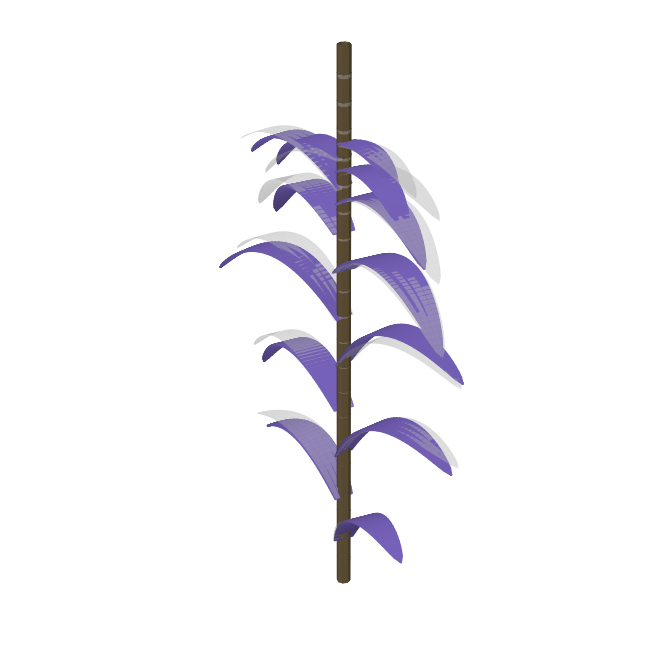
\includegraphics[width=1.1000in, height=1.1000in]{Figures/teaser/m_recipe.png}};
\node[tcap] at (1058.0,308.0) {\textcolor{uTxI}{\textbf{purple}: written by CropCode}\quad grey: the true plant};
\end{tikzpicture}
} (needs \usetikzlibrary{arrows.meta}).
\definecolor{tInk}{HTML}{1D221C}\definecolor{tMuted}{HTML}{5F685C}%
\definecolor{uRgbE}{HTML}{809EC2}\definecolor{uRgbF}{HTML}{E6ECF3}\definecolor{uRgbI}{HTML}{3F5F8F}%
\definecolor{uPcF}{HTML}{F6E9ED}\definecolor{uDepF}{HTML}{FAF2D4}%
\definecolor{uTxE}{HTML}{9D8CC4}\definecolor{uTxF}{HTML}{EAE7F2}\definecolor{uTxI}{HTML}{5E4A96}%
\definecolor{uOutE}{HTML}{B4B4B8}\definecolor{uArrow}{HTML}{8C8C8C}\definecolor{uModE}{HTML}{9A9A9A}%
\pgfdeclarehorizontalshading{uggband}{100bp}{color(0bp)=(uRgbF); color(30bp)=(uRgbF); color(45bp)=(uDepF); color(60bp)=(uPcF); color(75bp)=(uTxF); color(100bp)=(uTxF)}%
\begin{tikzpicture}[x=0.005in, y=-0.005in]
\useasboundingbox (0,0) rectangle (1320,340);
\tikzset{hdr/.style={anchor=center, inner sep=0, align=center, font={\fontsize{8.5}{10.2}\selectfont\sffamily\bfseries}},
         sp/.style={anchor=base, inner sep=0, align=center, text=tInk, font={\fontsize{7.2}{8.6}\selectfont\sffamily\bfseries}},
         tcap/.style={anchor=north, inner sep=0, align=center, text=tMuted, font={\fontsize{5.6}{6.8}\selectfont\sffamily}},
         blk/.style={color=uArrow, line width=3.0pt, -{Triangle[length=5.5pt,width=8.5pt]}}}
% ---- headers ----
\node[hdr, text=uRgbI] at (260.0,18.0) {Image of an occluded crop row (input)};
\node[hdr, text=tInk] at (662.0,18.0) {Model};
\node[hdr, text=uTxI] at (1055.0,18.0) {Procedural parameters of the center plant};
% ---- inputs: the row photographs ----
\node[sp] at (136.0,56.0) {sorghum};
\node[sp] at (384.0,56.0) {maize};
\draw[draw=uRgbE, line width=1.0pt, rounded corners=6.5pt, fill=uRgbF, dash pattern=on 3pt off 2pt] (20.0,68.0) rectangle (252.0,300.0);
\node[anchor=north west, inner sep=0] at (26.0,74.0) {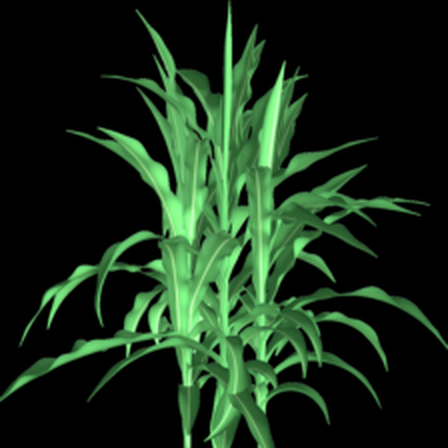
\includegraphics[width=1.1000in, height=1.1000in]{Figures/teaser/s_rgb.png}};
\draw[draw=white, densely dashed, line width=0.80pt] (104.0,88.0) rectangle (168.0,284.0);
\node[anchor=north west, inner sep=1.5pt, text=white, font={\fontsize{5.0}{6.0}\selectfont\sffamily\bfseries}] at (104.0,88.0) {target plant};
\node[tcap] at (136.0,308.0) {25\,\% hidden by neighbours};
\draw[draw=uRgbE, line width=1.0pt, rounded corners=6.5pt, fill=uRgbF, dash pattern=on 3pt off 2pt] (268.0,68.0) rectangle (500.0,300.0);
\node[anchor=north west, inner sep=0] at (274.0,74.0) {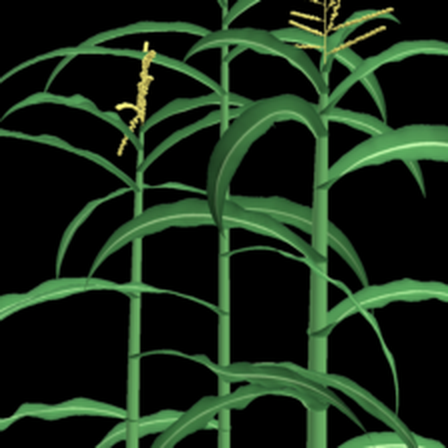
\includegraphics[width=1.1000in, height=1.1000in]{Figures/teaser/m_rgb.png}};
\draw[draw=white, densely dashed, line width=0.80pt] (354.0,84.0) rectangle (430.0,290.0);
\node[anchor=north west, inner sep=1.5pt, text=white, font={\fontsize{4.6}{5.6}\selectfont\sffamily\bfseries}] at (354.0,84.0) {target plant};
\node[tcap] at (384.0,308.0) {22\,\% hidden by neighbours};
\draw[blk] (510.0,184.0) -- (566.0,184.0);
% ---- the model ----
\draw[draw=uModE, line width=1.0pt, rounded corners=8.6pt, shading=uggband, shading angle=0] (574.0,68.0) rectangle (750.0,300.0);
\node[anchor=center, inner sep=0, text=tInk, font={\fontsize{9.0}{10.8}\selectfont\sffamily\bfseries}] at (662.0,120.0) {CropCode};
\draw[draw=uModE, line width=0.6pt, dash pattern=on 2.2pt off 1.6pt] (600.0,146.0) -- (724.0,146.0);
\node[anchor=north, inner sep=0, align=center, text=tInk, font={\fontsize{5.3}{6.6}\selectfont\sffamily}] at (662.0,166.0) {any-to-any\\autoencoder over\\photographs, depth,\\clouds and recipes;\\pretrained on single\\plants, fine-tuned\\on crop rows};
\draw[blk] (758.0,184.0) -- (806.0,184.0);
% ---- outputs: the procedural parameters ----
\draw[draw=uOutE, line width=0.9pt, rounded corners=8.6pt] (814.0,34.0) rectangle (1302.0,334.0);
\node[sp] at (938.0,56.0) {sorghum};
\node[sp] at (1178.0,56.0) {maize};
\draw[draw=uTxE, line width=1.0pt, rounded corners=6.5pt, fill=uTxF] (822.0,68.0) rectangle (1054.0,300.0);
\node[anchor=north west, inner sep=0] at (828.0,74.0) {
\includegraphics[width=1.1000in, height=1.1000in]{Figures/teaser/s_recipe.png}};
\draw[draw=uTxE, line width=1.0pt, rounded corners=6.5pt, fill=uTxF] (1062.0,68.0) rectangle (1294.0,300.0);
\node[anchor=north west, inner sep=0] at (1068.0,74.0) {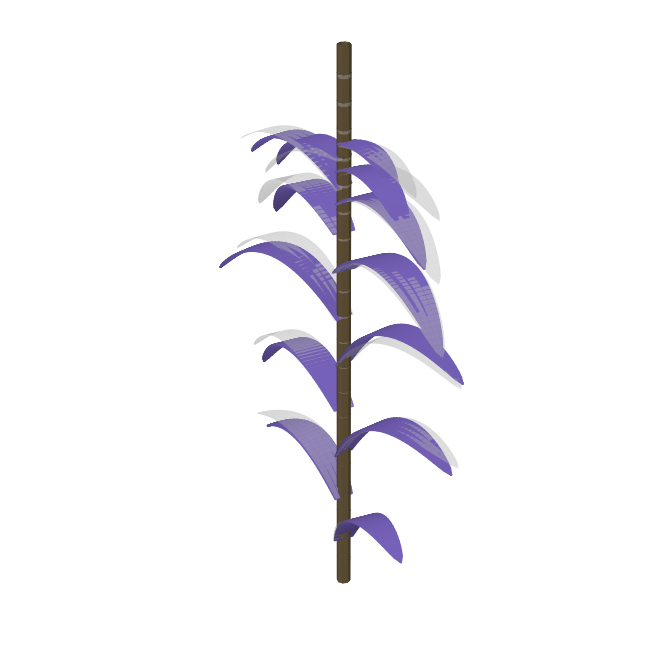
\includegraphics[width=1.1000in, height=1.1000in]{Figures/teaser/m_recipe.png}};
\node[tcap] at (1058.0,308.0) {\textcolor{uTxI}{\textbf{purple}: written by CropCode}\quad grey: the true plant};
\end{tikzpicture}
} (needs \usetikzlibrary{arrows.meta}).
\definecolor{tInk}{HTML}{1D221C}\definecolor{tMuted}{HTML}{5F685C}%
\definecolor{uRgbE}{HTML}{809EC2}\definecolor{uRgbF}{HTML}{E6ECF3}\definecolor{uRgbI}{HTML}{3F5F8F}%
\definecolor{uPcF}{HTML}{F6E9ED}\definecolor{uDepF}{HTML}{FAF2D4}%
\definecolor{uTxE}{HTML}{9D8CC4}\definecolor{uTxF}{HTML}{EAE7F2}\definecolor{uTxI}{HTML}{5E4A96}%
\definecolor{uOutE}{HTML}{B4B4B8}\definecolor{uArrow}{HTML}{8C8C8C}\definecolor{uModE}{HTML}{9A9A9A}%
\pgfdeclarehorizontalshading{uggband}{100bp}{color(0bp)=(uRgbF); color(30bp)=(uRgbF); color(45bp)=(uDepF); color(60bp)=(uPcF); color(75bp)=(uTxF); color(100bp)=(uTxF)}%
\begin{tikzpicture}[x=0.005in, y=-0.005in]
\useasboundingbox (0,0) rectangle (1320,340);
\tikzset{hdr/.style={anchor=center, inner sep=0, align=center, font={\fontsize{8.5}{10.2}\selectfont\sffamily\bfseries}},
         sp/.style={anchor=base, inner sep=0, align=center, text=tInk, font={\fontsize{7.2}{8.6}\selectfont\sffamily\bfseries}},
         tcap/.style={anchor=north, inner sep=0, align=center, text=tMuted, font={\fontsize{5.6}{6.8}\selectfont\sffamily}},
         blk/.style={color=uArrow, line width=3.0pt, -{Triangle[length=5.5pt,width=8.5pt]}}}
% ---- headers ----
\node[hdr, text=uRgbI] at (260.0,18.0) {Image of an occluded crop row (input)};
\node[hdr, text=tInk] at (662.0,18.0) {Model};
\node[hdr, text=uTxI] at (1055.0,18.0) {Procedural parameters of the center plant};
% ---- inputs: the row photographs ----
\node[sp] at (136.0,56.0) {sorghum};
\node[sp] at (384.0,56.0) {maize};
\draw[draw=uRgbE, line width=1.0pt, rounded corners=6.5pt, fill=uRgbF, dash pattern=on 3pt off 2pt] (20.0,68.0) rectangle (252.0,300.0);
\node[anchor=north west, inner sep=0] at (26.0,74.0) {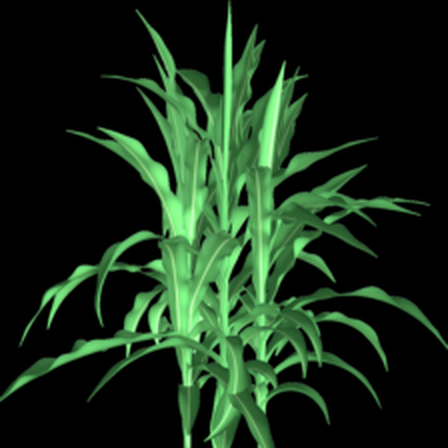
\includegraphics[width=1.1000in, height=1.1000in]{Figures/teaser/s_rgb.png}};
\draw[draw=white, densely dashed, line width=0.80pt] (104.0,88.0) rectangle (168.0,284.0);
\node[anchor=north west, inner sep=1.5pt, text=white, font={\fontsize{5.0}{6.0}\selectfont\sffamily\bfseries}] at (104.0,88.0) {target plant};
\node[tcap] at (136.0,308.0) {25\,\% hidden by neighbours};
\draw[draw=uRgbE, line width=1.0pt, rounded corners=6.5pt, fill=uRgbF, dash pattern=on 3pt off 2pt] (268.0,68.0) rectangle (500.0,300.0);
\node[anchor=north west, inner sep=0] at (274.0,74.0) {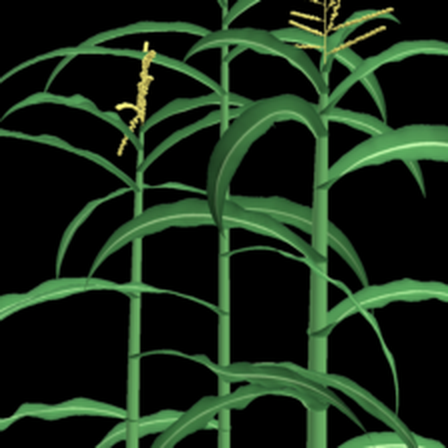
\includegraphics[width=1.1000in, height=1.1000in]{Figures/teaser/m_rgb.png}};
\draw[draw=white, densely dashed, line width=0.80pt] (354.0,84.0) rectangle (430.0,290.0);
\node[anchor=north west, inner sep=1.5pt, text=white, font={\fontsize{4.6}{5.6}\selectfont\sffamily\bfseries}] at (354.0,84.0) {target plant};
\node[tcap] at (384.0,308.0) {22\,\% hidden by neighbours};
\draw[blk] (510.0,184.0) -- (566.0,184.0);
% ---- the model ----
\draw[draw=uModE, line width=1.0pt, rounded corners=8.6pt, shading=uggband, shading angle=0] (574.0,68.0) rectangle (750.0,300.0);
\node[anchor=center, inner sep=0, text=tInk, font={\fontsize{9.0}{10.8}\selectfont\sffamily\bfseries}] at (662.0,120.0) {CropCode};
\draw[draw=uModE, line width=0.6pt, dash pattern=on 2.2pt off 1.6pt] (600.0,146.0) -- (724.0,146.0);
\node[anchor=north, inner sep=0, align=center, text=tInk, font={\fontsize{5.3}{6.6}\selectfont\sffamily}] at (662.0,166.0) {any-to-any\\autoencoder over\\photographs, depth,\\clouds and recipes;\\pretrained on single\\plants, fine-tuned\\on crop rows};
\draw[blk] (758.0,184.0) -- (806.0,184.0);
% ---- outputs: the procedural parameters ----
\draw[draw=uOutE, line width=0.9pt, rounded corners=8.6pt] (814.0,34.0) rectangle (1302.0,334.0);
\node[sp] at (938.0,56.0) {sorghum};
\node[sp] at (1178.0,56.0) {maize};
\draw[draw=uTxE, line width=1.0pt, rounded corners=6.5pt, fill=uTxF] (822.0,68.0) rectangle (1054.0,300.0);
\node[anchor=north west, inner sep=0] at (828.0,74.0) {
\includegraphics[width=1.1000in, height=1.1000in]{Figures/teaser/s_recipe.png}};
\draw[draw=uTxE, line width=1.0pt, rounded corners=6.5pt, fill=uTxF] (1062.0,68.0) rectangle (1294.0,300.0);
\node[anchor=north west, inner sep=0] at (1068.0,74.0) {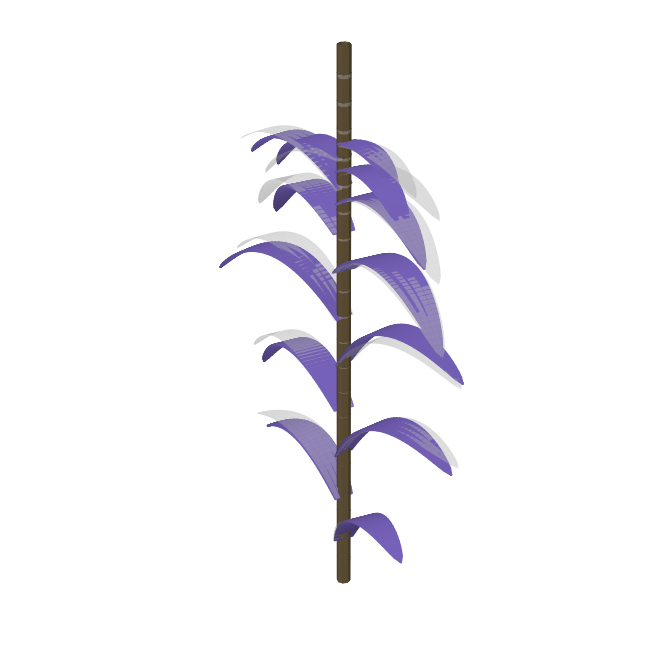
\includegraphics[width=1.1000in, height=1.1000in]{Figures/teaser/m_recipe.png}};
\node[tcap] at (1058.0,308.0) {\textcolor{uTxI}{\textbf{purple}: written by CropCode}\quad grey: the true plant};
\end{tikzpicture}
} (needs \usetikzlibrary{arrows.meta}).
\definecolor{tInk}{HTML}{1D221C}\definecolor{tMuted}{HTML}{5F685C}%
\definecolor{uRgbE}{HTML}{809EC2}\definecolor{uRgbF}{HTML}{E6ECF3}\definecolor{uRgbI}{HTML}{3F5F8F}%
\definecolor{uPcF}{HTML}{F6E9ED}\definecolor{uDepF}{HTML}{FAF2D4}%
\definecolor{uTxE}{HTML}{9D8CC4}\definecolor{uTxF}{HTML}{EAE7F2}\definecolor{uTxI}{HTML}{5E4A96}%
\definecolor{uOutE}{HTML}{B4B4B8}\definecolor{uArrow}{HTML}{8C8C8C}\definecolor{uModE}{HTML}{9A9A9A}%
\pgfdeclarehorizontalshading{uggband}{100bp}{color(0bp)=(uRgbF); color(30bp)=(uRgbF); color(45bp)=(uDepF); color(60bp)=(uPcF); color(75bp)=(uTxF); color(100bp)=(uTxF)}%
\begin{tikzpicture}[x=0.005in, y=-0.005in]
\useasboundingbox (0,0) rectangle (1320,340);
\tikzset{hdr/.style={anchor=center, inner sep=0, align=center, font={\fontsize{8.5}{10.2}\selectfont\sffamily\bfseries}},
         sp/.style={anchor=base, inner sep=0, align=center, text=tInk, font={\fontsize{7.2}{8.6}\selectfont\sffamily\bfseries}},
         tcap/.style={anchor=north, inner sep=0, align=center, text=tMuted, font={\fontsize{5.6}{6.8}\selectfont\sffamily}},
         blk/.style={color=uArrow, line width=3.0pt, -{Triangle[length=5.5pt,width=8.5pt]}}}
% ---- headers ----
\node[hdr, text=uRgbI] at (260.0,18.0) {Image of an occluded crop row (input)};
\node[hdr, text=tInk] at (662.0,18.0) {Model};
\node[hdr, text=uTxI] at (1055.0,18.0) {Procedural parameters of the center plant};
% ---- inputs: the row photographs ----
\node[sp] at (136.0,56.0) {sorghum};
\node[sp] at (384.0,56.0) {maize};
\draw[draw=uRgbE, line width=1.0pt, rounded corners=6.5pt, fill=uRgbF, dash pattern=on 3pt off 2pt] (20.0,68.0) rectangle (252.0,300.0);
\node[anchor=north west, inner sep=0] at (26.0,74.0) {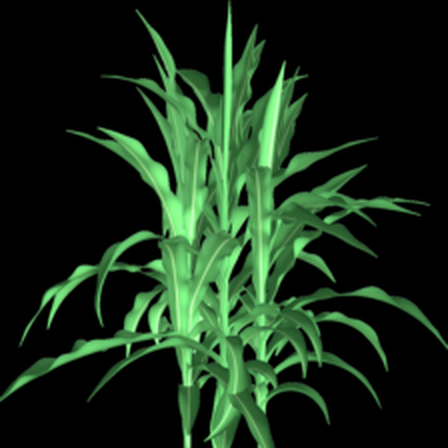
\includegraphics[width=1.1000in, height=1.1000in]{Figures/teaser/s_rgb.png}};
\draw[draw=white, densely dashed, line width=0.80pt] (104.0,88.0) rectangle (168.0,284.0);
\node[anchor=north west, inner sep=1.5pt, text=white, font={\fontsize{5.0}{6.0}\selectfont\sffamily\bfseries}] at (104.0,88.0) {target plant};
\node[tcap] at (136.0,308.0) {25\,\% hidden by neighbours};
\draw[draw=uRgbE, line width=1.0pt, rounded corners=6.5pt, fill=uRgbF, dash pattern=on 3pt off 2pt] (268.0,68.0) rectangle (500.0,300.0);
\node[anchor=north west, inner sep=0] at (274.0,74.0) {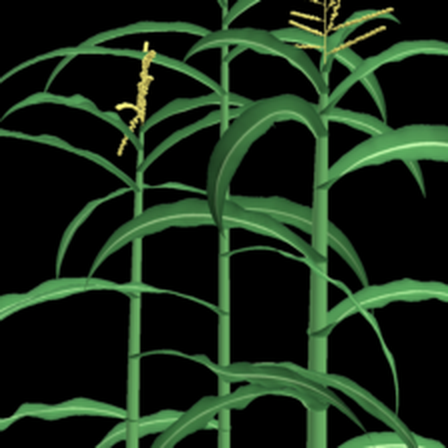
\includegraphics[width=1.1000in, height=1.1000in]{Figures/teaser/m_rgb.png}};
\draw[draw=white, densely dashed, line width=0.80pt] (354.0,84.0) rectangle (430.0,290.0);
\node[anchor=north west, inner sep=1.5pt, text=white, font={\fontsize{4.6}{5.6}\selectfont\sffamily\bfseries}] at (354.0,84.0) {target plant};
\node[tcap] at (384.0,308.0) {22\,\% hidden by neighbours};
\draw[blk] (510.0,184.0) -- (566.0,184.0);
% ---- the model ----
\draw[draw=uModE, line width=1.0pt, rounded corners=8.6pt, shading=uggband, shading angle=0] (574.0,68.0) rectangle (750.0,300.0);
\node[anchor=center, inner sep=0, text=tInk, font={\fontsize{9.0}{10.8}\selectfont\sffamily\bfseries}] at (662.0,120.0) {CropCode};
\draw[draw=uModE, line width=0.6pt, dash pattern=on 2.2pt off 1.6pt] (600.0,146.0) -- (724.0,146.0);
\node[anchor=north, inner sep=0, align=center, text=tInk, font={\fontsize{5.3}{6.6}\selectfont\sffamily}] at (662.0,166.0) {any-to-any\\autoencoder over\\photographs, depth,\\clouds and recipes;\\pretrained on single\\plants, fine-tuned\\on crop rows};
\draw[blk] (758.0,184.0) -- (806.0,184.0);
% ---- outputs: the procedural parameters ----
\draw[draw=uOutE, line width=0.9pt, rounded corners=8.6pt] (814.0,34.0) rectangle (1302.0,334.0);
\node[sp] at (938.0,56.0) {sorghum};
\node[sp] at (1178.0,56.0) {maize};
\draw[draw=uTxE, line width=1.0pt, rounded corners=6.5pt, fill=uTxF] (822.0,68.0) rectangle (1054.0,300.0);
\node[anchor=north west, inner sep=0] at (828.0,74.0) {
\includegraphics[width=1.1000in, height=1.1000in]{Figures/teaser/s_recipe.png}};
\draw[draw=uTxE, line width=1.0pt, rounded corners=6.5pt, fill=uTxF] (1062.0,68.0) rectangle (1294.0,300.0);
\node[anchor=north west, inner sep=0] at (1068.0,74.0) {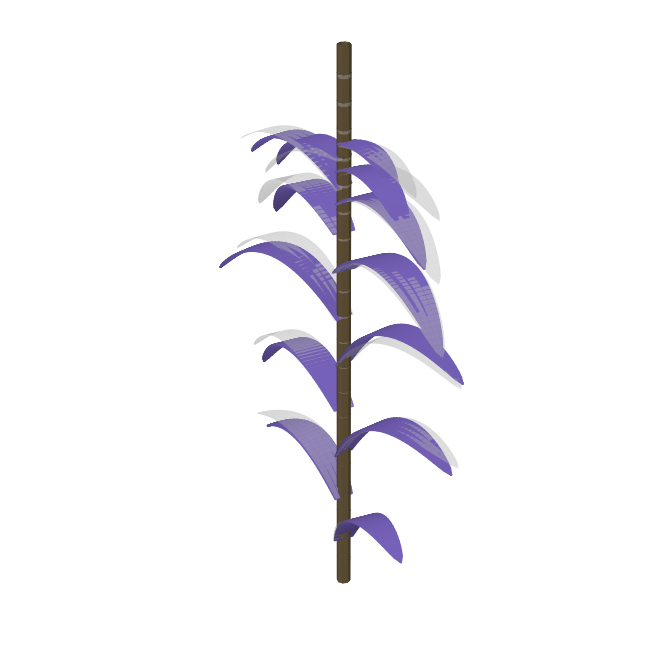
\includegraphics[width=1.1000in, height=1.1000in]{Figures/teaser/m_recipe.png}};
\node[tcap] at (1058.0,308.0) {\textcolor{uTxI}{\textbf{purple}: written by CropCode}\quad grey: the true plant};
\end{tikzpicture}
